% Provenance (never printed): old terminale S material on the continental crust
% (granitic composition, thickness, density, age; roots and isostasy). Thickness
% from Christensen-Mooney 1995 and Cogley 1984 (CRUST1.0 dropped: no licence,
% Sync 1); ocean-floor ages from figdata/grade-12/crust_ages.py (Seton 2020 grid,
% as in g11.01). Airy isostasy is g11.03's: recalled, not re-derived. Radiometric
% dating is g12.07's: ages are only quoted here.
\chapter{Kerak Benua}\label{ch:g12:continental-crust}

Di barat laut Kanada, di dekat Sungai Acasta, tersingkap batuan kelabu yang
bergaris-garis dengan pita terang dan gelap. Umurnya telah ditentukan 4.00
sampai 4.03 miliar tahun: gneis Acasta, batuan tertua yang diketahui. Yang lebih
tua lagi adalah butir-butir mineral zirkon, masing-masing sepanjang sepersekian
milimeter, yang ditemukan dalam batuan sedimen tua di Jack Hills, Australia
Barat. Terkikis dari batuan yang lebih tua dan terbawa air sebelum terkubur,
butir-butir itu mengkristal 4.4 miliar tahun yang lalu, dan menunjukkan bahwa
kerak sudah ada saat itu. Tidak ada dasar samudra yang umurnya bahkan
seperdua puluh umur itu. Bab ini menanyakan dari apa benua-benua tersusun, dan
mengapa benua-benua itu bertahan.
% ledger: bowring99:acasta, wilde01:zircon, uw14:jack-hills, photo:g12-acasta, photo:g12-jack-hills-zircons

\begin{omfigure}
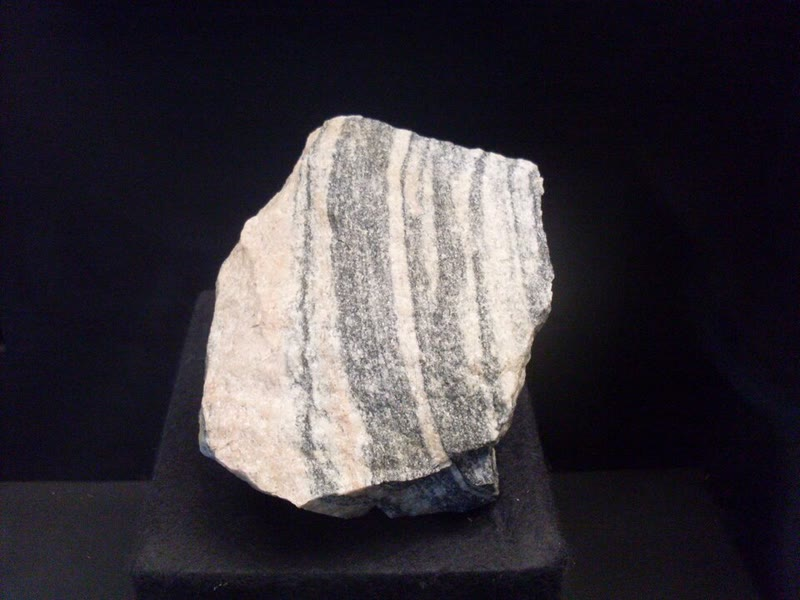
\includegraphics[height=4.6cm]{images/book2/g12-pedro-acasta-gneiss.jpg}\hspace{0.04\linewidth}%
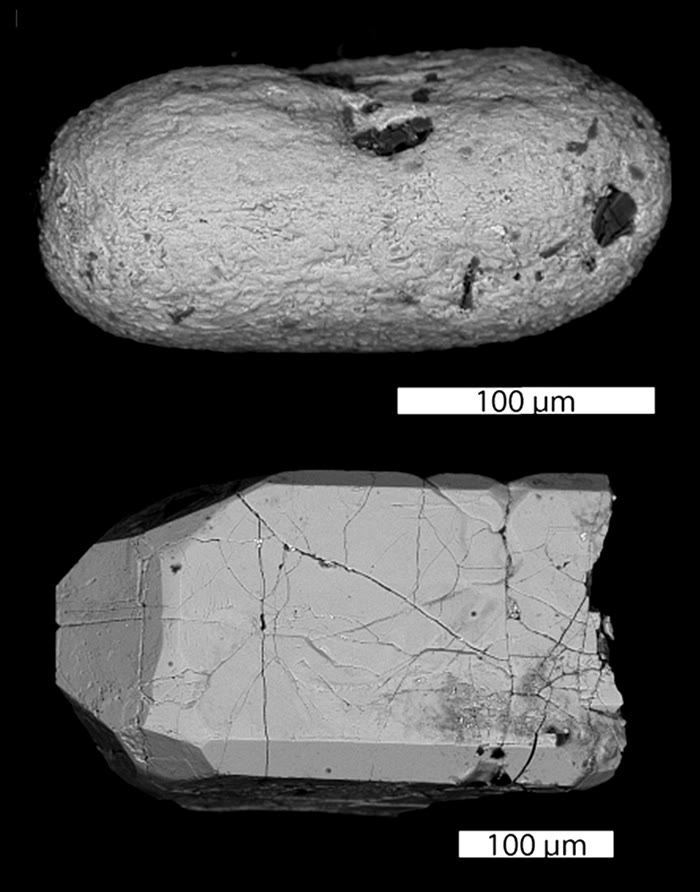
\includegraphics[height=4.6cm]{images/book2/g12-cavosie-jack-hills-zircons.jpg}

{\small Kiri: sepotong gneis Acasta, berumur 4.03 miliar tahun, dalam sebuah
pameran museum. Foto Pedroalexandrade (CC~BY-SA~3.0). Kanan: dua butir zirkon
dari Jack Hills, Australia Barat, yang dilihat dengan mikroskop elektron;
setiap batang skala panjangnya \qty{100}{\micro m}. Butir yang atas menjadi
bulat ketika terbawa air, yang bawah mempertahankan bidang-bidang kristalnya.
Citra A.~Cavosie dan J.~Valley (domain publik).}
\end{omfigure}
% ledger: photo:g12-acasta, photo:g12-jack-hills-zircons

\begin{recall}
Kerak berakhir di \omterm{def:g11:seismic-structure:moho}{Moho}, yang di bawahnya terdapat mantel yang lebih rapat
(\cref{ch:g11:seismic-structure}). \omterm{def:g11:ocean-ridges:oceanic-lithosphere}{Kerak samudra} adalah lapisan basalt dan \omterm{def:g11:ocean-ridges:gabbro}{gabro}
setebal sekitar \qty{7}{km} yang dibuat di punggungan
(\cref{ch:g11:ocean-ridges}), dan umurnya tidak pernah lebih dari sekitar 190
juta tahun (\cref{ch:g11:drift-to-spreading}). Lapisan-lapisan luar mengapung
di atas \omterm{def:g11:lithosphere-asthenosphere:lithosphere}{astenosfer}: dalam model Airy, wilayah yang permukaannya lebih tinggi
sebesar $h$ mempunyai kerak yang lebih tebal sebesar $h\,\rho_m/(\rho_m -
\rho_c)$ (\cref{ch:g11:lithosphere-asthenosphere}). Batuan beku dinamai
menurut \omterm{def:g11:igneous-rocks:texture}{tekstur} dan kandungan silikanya: \omterm{def:g11:igneous-rocks:felsic-mafic}{mafik} dari 45 sampai
\qty{55}{\percent} \ce{SiO2}, \omterm{def:g11:igneous-rocks:felsic-mafic}{intermediet} dari 55 sampai 65, \omterm{def:g11:igneous-rocks:felsic-mafic}{felsik} dari 65
sampai 75 (\cref{ch:g11:igneous-rocks}). Unsur radioaktif meluruh dengan laju
yang tetap, dan itulah yang memberi batuan umurnya (buku-buku fisika;
\cref{ch:g12:age-of-the-earth}).
\end{recall}
% ledger: white92:crust, data:b2-seafloor-age, tulane:magma-types

\section{Dari apa benua-benua tersusun}

\begin{definition}[Kerak benua]\label{def:g12:continental-crust:continental-crust}
Yang disebut \emph{kerak benua}\index{kerak benua} adalah kerak yang membentuk
benua-benua, termasuk bagian-bagiannya yang berada di bawah laut dangkal. Kerak
itu tebal, rata-rata berkomposisi granitik di bagian atasnya, ringan, dan dapat
sangat tua.
\end{definition}
% ledger: tulane:crust-types, tulane:roots, cogley84:continents

Benua-benua lebih luas daripada daratan. Tepi-tepi \omterm{def:g12:continental-crust:continental-crust}{kerak benua} terletak di bawah
laut, pada paparan benua: bila dipetakan dengan cara ini, \omterm{def:g12:continental-crust:continental-crust}{kerak benua} menutupi
\num{210}~juta~\unit{km^2}, \qty{41}{\percent} dari permukaan Bumi, dan hampir
sepertiganya, \qty{30.6}{\percent}, terendam. Bila bagian-bagiannya yang
terendam ikut dihitung, tinggi rata-rata \omterm{def:g12:continental-crust:continental-crust}{kerak benua} hanya sekitar
\qty{120}{m} di atas permukaan laut.
% ledger: cogley84:continents

Di permukaan, benua-benua memperlihatkan segala jenis batuan --- sedimen,
\omterm{def:g11:igneous-rocks:volcanic-plutonic}{batuan vulkanik}, batuan metamorf --- tetapi di bawah selimut sedimennya, \omterm{def:g12:continental-crust:continental-crust}{kerak
benua} sebagian besar tersusun dari batuan granitik serta batuan metamorf dan
\omterm{def:g11:igneous-rocks:volcanic-plutonic}{plutonik} dari \omterm{def:g12:continental-crust:root}{akar-akar} pegunungan tua. Rata-rata, seluruh \omterm{def:g12:continental-crust:continental-crust}{kerak benua}
mengandung \qty{60.6}{\percent} silika; bagian atasnya lebih kaya,
\qty{66.6}{\percent}, sehingga bagian dalamnya pasti lebih miskin.
% ledger: rg14:crust, tulane:crust-types, cm95:crust

\begin{omfigure}
\begin{tikzpicture}
\begin{axis}[omrecord, ybar=0pt, width=0.92\linewidth, height=5.0cm, bar width=7pt,
  ymin=0, ymax=80, ylabel={fraksi massa (\unit{\percent})},
  symbolic x coords={SiO2, Al2O3, FeO, MgO, CaO, Na2O, K2O},
  xticklabels={\ce{SiO2}, \ce{Al2O3}, \ce{FeO}, \ce{MgO}, \ce{CaO}, \ce{Na2O}, \ce{K2O}},
  xtick=data, enlarge x limits=0.08, ymajorgrids=true, xmajorgrids=false,
  legend style={font=\scriptsize, at={(0.98,0.97)}, anchor=north east, legend columns=1}]
% ledger: rg14:crust (upper and bulk continental crust; FeO* total iron)
\addplot[fill=omLithGranite, draw=black!60] coordinates {(SiO2,66.6) (Al2O3,15.4) (FeO,5.04) (MgO,2.48) (CaO,3.59) (Na2O,3.27) (K2O,2.80)};
\addplot[fill=omProp!55, draw=black!60] coordinates {(SiO2,60.6) (Al2O3,15.9) (FeO,6.71) (MgO,4.66) (CaO,6.41) (Na2O,3.07) (K2O,1.81)};
% ledger: earle:magma-oxides (mafic magma: midpoint of each range, the bar spans the range)
\addplot[fill=omLithBasalt, draw=black!60, error bars/.cd, y dir=both, y explicit]
  coordinates {(SiO2,50) +- (0,5) (Al2O3,16) +- (0,2) (FeO,10) +- (0,2) (MgO,7) +- (0,2) (CaO,9) +- (0,2) (Na2O,2) +- (0,1) (K2O,1.75) +- (0,1.25)};
\legend{kerak benua bagian atas, seluruh kerak benua, magma mafik (rentang)}
\end{axis}
\end{tikzpicture}

{\small Komposisi \omterm{def:g12:continental-crust:continental-crust}{kerak benua} dibandingkan dengan magma \omterm{def:g11:igneous-rocks:felsic-mafic}{mafik}, jenis magma yang
membentuk \omterm{def:g11:ocean-ridges:oceanic-lithosphere}{kerak samudra}: oksida-oksida utama, dalam persen massa (\ce{FeO}
menghitung seluruh besi). \omterm{def:g12:continental-crust:continental-crust}{Kerak benua} lebih kaya silika, natrium, dan kalium,
dan lebih miskin besi, magnesium, dan kalsium. Data: Rudnick dan Gao (2014);
rentang magma \omterm{def:g11:igneous-rocks:felsic-mafic}{mafik} dari S.~Earle, \emph{Physical Geology} (CC~BY~4.0).}
\end{omfigure}
% ledger: rg14:crust, earle:magma-oxides

\section{Kerak yang tebal dan ringan}

Survei seismik menemukan \omterm{def:g11:seismic-structure:moho}{Moho} di bawah benua-benua pada kedalaman yang sangat
berbeda-beda. Dirata-ratakan atas semua benua, dengan bobot luas, kerak itu
tebalnya sekitar \qty{41}{km}; kerak itu lebih tipis, sekitar \qty{30}{km}, di
tempat kerak telah teregang, dan lebih tebal, rata-rata sekitar \qty{46}{km},
di sabuk-sabuk pegunungan. Jauh dari sabuk pegunungan, tebalnya umumnya 35
sampai \qty{40}{km}; di bawah pegunungan yang tertinggi, 50 sampai
\qty{70}{km}, sekitar \qty{70}{km} di bawah sebagian Tibet. \omterm{def:g11:ocean-ridges:oceanic-lithosphere}{Kerak samudra}
tebalnya sekitar \qty{7}{km}: \omterm{def:g12:continental-crust:continental-crust}{kerak benua} lima sampai sepuluh kali lebih tebal.
% ledger: cm95:crust, tulane:roots, karplus:tibet-moho, white92:crust

\begin{omfigure}
\begin{tikzpicture}
\begin{axis}[omrecord, xbar, bar shift=0pt, width=0.78\linewidth, height=5.0cm, bar width=8pt,
  xmin=0, xmax=80, ymin=0.4, ymax=5.6, ytick={1,...,5},
  yticklabels={kerak samudra, benua yang teregang, benua (rata-rata), pegunungan (rata-rata), di bawah Tibet},
  xlabel={tebal kerak (\unit{km})}, ymajorgrids=false,
  nodes near coords, nodes near coords style={font=\scriptsize, anchor=west}, point meta=explicit symbolic]
% ledger: white92:crust, cm95:crust, karplus:tibet-moho
\addplot[fill=omLithBasalt, draw=black!60] coordinates {(7.1,1) [7.1]};
\addplot[fill=omLithGranite, draw=black!60] coordinates {(30.5,2) [30.5] (41.1,3) [41.1] (46.3,4) [46.3] (70,5) [sekitar 70]};
\end{axis}
\end{tikzpicture}

{\small Tebal kerak dari pengukuran seismik. Data: White, McKenzie, dan O'Nions
(1992) untuk \omterm{def:g11:ocean-ridges:oceanic-lithosphere}{kerak samudra}; Christensen dan Mooney (1995) untuk rata-rata
benua; Karplus dan kawan-kawan (2019) untuk Tibet.}
\end{omfigure}
% ledger: white92:crust, cm95:crust, karplus:tibet-moho

\omterm{def:g12:continental-crust:continental-crust}{Kerak benua} juga ringan. Massa jenis rata-ratanya sekitar
\qty{2830}{kg/m^3}. Basalt dan \omterm{def:g11:ocean-ridges:gabbro}{gabro} \omterm{def:g11:ocean-ridges:oceanic-lithosphere}{kerak samudra}, yang kaya piroksen dan
olivin, mencapai sekitar \qty{3000}{kg/m^3} (\cref{ch:g11:minerals}), dan mantel
tepat di bawah \omterm{def:g11:seismic-structure:moho}{Moho} sekitar \qty{3380}{kg/m^3}. Kerak yang tebal dan ringan
mengapung tinggi: inilah sebabnya benua-benua berdiri di atas dasar samudra,
dan sebabnya sebuah benua tidak dapat diseret turun di \omterm{def:g11:subduction-zones:subduction}{zona subduksi}. Ketika
sebuah benua tiba di sebuah palung, benua itu terlalu ringan untuk tenggelam;
\omterm{def:g11:subduction-zones:subduction}{subduksi} berhenti, dan kedua benua bertumbukan
(\cref{ch:g12:mountain-building}). \omterm{def:g12:continental-crust:continental-crust}{Kerak benua}, sekali terbentuk, sulit
dihancurkan.
% ledger: cm95:crust, data:prem, tulane:roots, tulane:no-subduct
% values (mineral_density.py): basalt/gabbro rock line 3.0015 g/cm3

\begin{omfigure}
\begin{tikzpicture}[x=1cm, y=0.075cm, font=\footnotesize]
  % continental column: 41 km of crust, surface at +0.12 km (mean height); ocean column: 3.7 km of water drawn schematically
  \fill[omLithGranite] (0,0) rectangle (3,-41);
  \fill[omLithPeridotite!60] (0,-41) rectangle (3,-60);
  \fill[omSea] (6,0) rectangle (9,-4);
  \fill[omLithGabbro] (6,-4) rectangle (9,-11.1);
  \fill[omLithPeridotite!60] (6,-11.1) rectangle (9,-60);
  \draw[black!60] (0,0) rectangle (3,-60) (6,0) rectangle (9,-60);
  \draw[line width=0.9pt] (0,-41) -- (3,-41) (6,-11.1) -- (9,-11.1);
  \node[align=center] at (1.5,-20) {kerak benua\\sekitar \qty{41}{km}\\\qty{2830}{kg/m^3}\\sampai 4 miliar tahun};
  \node[align=center] at (7.5,-24) {mantel\\\qty{3380}{kg/m^3}\\di bawah Moho};
  \node[align=center] at (1.5,-50.5) {mantel};
  \node at (7.5,-2) {samudra};
  \draw[black!60] (8.6,-7.6) -- (9.3,-7.6);
  \node[anchor=west, align=left] at (9.3,-7.6) {kerak samudra, sekitar \qty{7}{km}\\\qty{3000}{kg/m^3}\\kurang dari 200 juta tahun};
  \node[anchor=east] at (-0.1,-41) {Moho};
  \node[anchor=east] at (5.9,-11.1) {Moho};
  \node[anchor=south] at (1.5,0) {sebuah benua};
  \node[anchor=south] at (7.5,0) {sebuah samudra};
  \foreach \d in {0,20,40,60} {\draw[black!60] (-1.5,-\d) -- (-1.3,-\d); \node[anchor=east, font=\scriptsize] at (-1.5,-\d) {\d};}
  \draw[black!60] (-1.4,0) -- (-1.4,-60);
  \node[rotate=90, font=\scriptsize] at (-2.3,-30) {kedalaman (\unit{km})};
\end{tikzpicture}

{\small Sebuah benua dan sebuah samudra berdampingan (kedalaman menurut skala,
lebar tidak; samudra digambar sedalam \qty{4}{km}): \omterm{def:g12:continental-crust:continental-crust}{kerak benua} lebih tebal,
lebih ringan, dan jauh lebih tua daripada \omterm{def:g11:ocean-ridges:oceanic-lithosphere}{kerak samudra}.}
\end{omfigure}
% ledger: cm95:crust, white92:crust, data:prem, bowring99:acasta, data:b2-seafloor-age

\begin{method}[Membandingkan kerak benua dan kerak samudra]\label{met:g12:continental-crust:compare}
Untuk mengetahui jenis kerak yang ada di bawah suatu tempat, bandingkan lima
sifat:
\begin{enumerate}
  \item tebal: sekitar \qty{7}{km} untuk \omterm{def:g11:ocean-ridges:oceanic-lithosphere}{kerak samudra}, 30 sampai
        \qty{70}{km} untuk \omterm{def:g12:continental-crust:continental-crust}{kerak benua};
  \item batuan: basalt dan \omterm{def:g11:ocean-ridges:gabbro}{gabro}, atau granit, gneis, dan kerabatnya, di
        bawah selimut sedimen;
  \item komposisi: sekitar \qty{50}{\percent} silika, atau sekitar 60 dan
        lebih;
  \item massa jenis: sekitar \qty{3000}{kg/m^3}, atau sekitar \qty{2830}{kg/m^3};
  \item umur: kurang dari 200 juta tahun, atau sampai 4 miliar tahun.
\end{enumerate}
Ketinggian adalah petunjuk, bukan uji: sebagian besar dasar samudra terletak
beberapa kilometer di bawah permukaan laut, tetapi tepi-tepi benua terletak di
bawah laut dangkal.
\end{method}
% ledger: white92:crust, cm95:crust, rg14:crust, earle:magma-oxides, cogley84:continents

\begin{example}[Dasar laut yang dangkal]\label{ex:g12:continental-crust:shelf}
Sebuah kapal survei menemukan dasar laut sedalam \qty{150}{m}. Profil seismik
menempatkan \omterm{def:g11:seismic-structure:moho}{Moho} \qty{32}{km} di bawah dasar laut; sebuah inti bor mengangkat,
dari bawah sedimen, batuan berbutir kasar yang tersusun dari kuarsa, feldspar,
dan mika. Kerak apa yang ada di sana?

\emph{Penyelesaian.} Tebalnya sekitar \qty{32}{km}: \omterm{def:g12:continental-crust:continental-crust}{kerak benua}, lebih tipis
daripada rata-rata, seperti di tempat kerak telah teregang. Granit di bawah
sedimen: \omterm{def:g12:continental-crust:continental-crust}{kerak benua}. Dasar laut itu adalah paparan benua, salah satu bagian
terendam yang meliputi hampir sepertiga benua-benua.
\end{example}
% invented numbers; ledger: cm95:crust, cogley84:continents

Seberapa berat seluruh kerak ini? Lapisan yang tipis dibandingkan dengan jari-jari
Bumi mempunyai massa yang sederhana.

\begin{proposition}[Massa lapisan tipis]\label{prop:g12:continental-crust:thin-layer}
Lapisan yang tebalnya $H$ dan massa jenisnya $\rho$, yang menutupi fraksi $f$
dari permukaan sebuah planet berjari-jari $R \gg H$ dan bermassa jenis
rata-rata $\bar\rho$, mempunyai massa $m \approx 4\pi R^2 f H \rho$, dan
bagiannya dari massa planet $M$ adalah
\[
  \frac{m}{M} \approx 3 f\,\frac{H}{R}\,\frac{\rho}{\bar\rho}.
\]
\end{proposition}
% ledger: earth:Rmean, earth:density

\begin{proof}
Luas permukaan planet adalah $4\pi R^2$; lapisan itu menutupi $4\pi R^2 f$ dan,
karena tipis, mempunyai volume yang mendekati luas itu dikali $H$, sehingga $m \approx 4\pi R^2
f H \rho$. Massa planet adalah $M = \tfrac{4}{3}\pi R^3 \bar\rho$. Dengan
membaginya, $m/M \approx 4\pi R^2 f H \rho / (\tfrac{4}{3}\pi R^3 \bar\rho) = 3 f (H/R)
(\rho/\bar\rho)$.
\end{proof}

Untuk \omterm{def:g11:ocean-ridges:oceanic-lithosphere}{kerak samudra} --- \qty{59}{\percent} sisa permukaan,
\qty{7.1}{km}, sekitar \qty{3000}{kg/m^3} --- dengan $R = \qty{6371}{km}$ dan
$\bar\rho = \qty{5513}{kg/m^3}$, bagiannya adalah $3 \times 0.59 \times
(7.1/6371) \times (3000/5513) \approx 0.0011$: sekitar sepersepuluh persen
massa Bumi. Soal akhir pekan melakukan hal yang sama untuk benua-benua.
% ledger: cogley84:continents, white92:crust, earth:Rmean, earth:density

\section{Kerak yang tua}

Dasar samudra muda di mana-mana: tiga perempatnya lebih muda daripada 100 juta
tahun, dan hampir tidak ada yang lebih tua daripada 190 juta tahun. Benua-benua
lain halnya. Batuannya meliputi hampir seluruh sejarah Bumi, dari gneis
Acasta, yang berumur 4.03 miliar tahun, sampai lava yang meletus hari ini, dan
butir-butir zirkon membawa catatan itu mundur sampai 4.4 miliar tahun.
% ledger: data:b2-seafloor-age, bowring99:acasta, uw14:jack-hills

\begin{omfigure}
\begin{tikzpicture}
\begin{axis}[omrecord, ybar interval, width=0.82\linewidth, height=5.0cm,
  xmin=0, xmax=200, ymin=0, ymax=0.12, xtick={0,20,...,200},
  xlabel={umur dasar samudra (juta tahun)},
  ylabel={bagian dasar samudra}, yticklabel style={/pgf/number format/fixed},
  ymajorgrids=true, xmajorgrids=false, clip=false, x tick label as interval=false]
% computed in figdata/grade-12/crust_ages.py (Seton 2020 grid, 1-degree cells, area-weighted)
\addplot[fill=omDef!35, draw=omDef] table[x=age_lo, y=share] {figdata/out/grade-12-crust_ages-hist.dat};
\node[anchor=north east, align=right, font=\scriptsize, fill=white, inner sep=2pt] at (axis cs:198,0.115)
  {batuan benua tertua: \num{4030} juta tahun,\\dua puluh kali lebih tua daripada dasar samudra tertua};
\end{axis}
\end{tikzpicture}

{\small Seberapa tua dasar samudra: bagian luasnya dalam setiap pita 10 juta
tahun. Dasar yang muda mendominasi; hampir tidak ada yang lebih tua daripada 190
juta tahun (beberapa cekungan tua di Mediterania timur tidak diikutkan). Data:
Seton dan kawan-kawan (2020), dihitung.}
\end{omfigure}
% ledger: data:b2-seafloor-age, bowring99:acasta
% values (crust_ages.py): oldest_open_myr 192.5, share_younger_100 0.765, share_younger_150 0.956, rock_over_floor 20.9

Bagian-bagian benua yang tertua membentuk intinya.

\begin{definition}[Kraton]\label{def:g12:continental-crust:craton}
Yang disebut \emph{kraton}\index{kraton} adalah inti benua yang tua dan stabil:
\omterm{def:g12:continental-crust:continental-crust}{kerak benua} yang terbentuk dan terdeformasi lebih dari satu miliar tahun yang
lalu, yang sejak itu telah mendingin dan tidak lagi terdeformasi. Batuannya
sebagian besar batuan metamorf dan \omterm{def:g11:igneous-rocks:volcanic-plutonic}{plutonik}, \omterm{def:g12:continental-crust:root}{akar-akar} dalam pegunungan masa
lalu.
\end{definition}
% ledger: tulane:cratons

Di sekeliling \omterm{def:g12:continental-crust:craton}{kraton} terdapat sabuk-sabuk batuan terdeformasi yang lebih muda,
yaitu \omterm{def:g12:continental-crust:root}{akar-akar} tererosi dari pegunungan yang terbangun kemudian; sabuk-sabuk
itu cenderung makin muda ke arah tepi benua. Sebuah benua tumbuh melalui
pembentukan pegunungan yang mengelaskan kerak baru pada tepi-tepinya, di
sekeliling inti purba. Di Kanada, tempat batuan \omterm{def:g12:continental-crust:craton}{kraton} terletak di permukaan,
tersingkap gneis dan granit yang berumur 1 sampai 3 miliar tahun, seperti di
tepi danau ini.
% ledger: tulane:cratons, photo:g12-canadian-shield

\begin{omfigure}
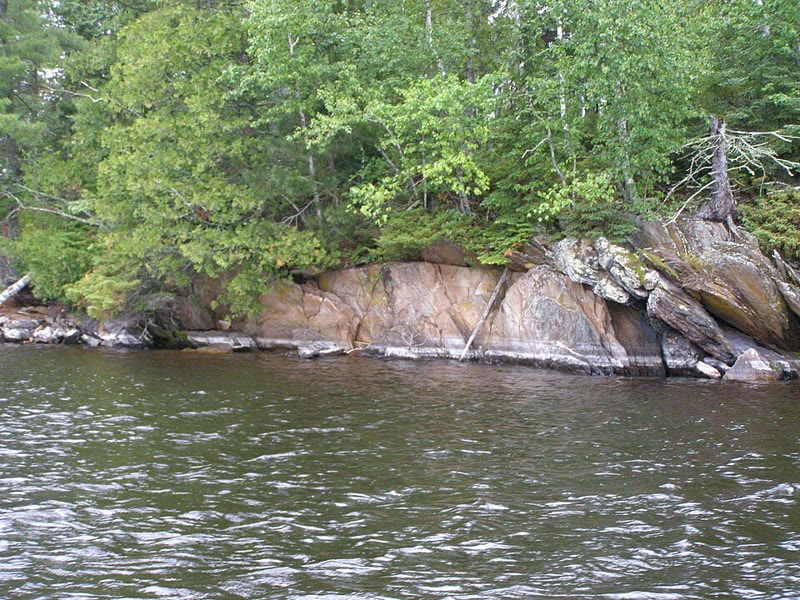
\includegraphics[height=5.0cm]{images/book2/g12-light-canadian-shield.jpg}

{\small Gneis dan granit yang berumur 1 sampai 3 miliar tahun di tepi sebuah
danau di Kanada, bagian dari inti purba Amerika Utara. Foto Chris Light
(CC~BY-SA~4.0).}
\end{omfigure}
% ledger: photo:g12-canadian-shield

Mengapa \omterm{def:g12:continental-crust:continental-crust}{kerak benua} bertahan, sedangkan dasar samudra selalu muda? \omterm{def:g11:ocean-ridges:oceanic-lithosphere}{Kerak
samudra} rapat: kerak itu tenggelam kembali ke dalam mantel di \omterm{def:g11:subduction-zones:subduction}{zona subduksi},
dan tidak satu bagian pun yang bertahan jauh lebih lama daripada 200 juta tahun.
\omterm{def:g12:continental-crust:continental-crust}{Kerak benua} terlalu ringan untuk tenggelam; kerak itu dapat dikikis oleh erosi,
diregangkan, atau dikerutkan, tetapi tetap berada di permukaan. Batuan sebuah
benua adalah arsip empat miliar tahun.
% ledger: tulane:no-subduct, tulane:roots, data:b2-seafloor-age

\section{Akar pegunungan}

Makin tinggi pegunungan, makin tebal kerak di bawahnya.

\begin{definition}[Akar pegunungan]\label{def:g12:continental-crust:root}
Yang disebut \emph{akar}\index{akar (pegunungan)} sebuah pegunungan adalah
bagian dari keraknya yang menebal yang menjulur ke bawah ke dalam mantel, di
bawah aras \omterm{def:g11:seismic-structure:moho}{Moho} di bawah dataran rendah di sekitarnya.
\end{definition}
% ledger: tulane:roots

Model Airy meramalkan \omterm{def:g12:continental-crust:root}{akar} itu: pegunungan yang berdiri setinggi $h$ di atas
sekitarnya mempunyai \omterm{def:g12:continental-crust:root}{akar} $r = h\,\rho_c/(\rho_m - \rho_c)$, sekitar lima kali
tingginya dengan $\rho_c = \qty{2830}{kg/m^3}$ dan $\rho_m =
\qty{3380}{kg/m^3}$ (\cref{prop:g11:lithosphere-asthenosphere:airy}). Dua
jenis pengukuran melihat \omterm{def:g12:continental-crust:root}{akar-akar} itu. Survei seismik menemukan \omterm{def:g11:seismic-structure:moho}{Moho} lebih
dalam di bawah pegunungan: 50 sampai \qty{70}{km} di bawah banyak sabuk
pegunungan, sekitar \qty{70}{km} di bawah sebagian Tibet. Gravitasi di atas
pegunungan lebih lemah daripada yang diperkirakan dari massanya yang tampak:
\omterm{def:g12:continental-crust:root}{akar} yang ringan, yang menempati tempat mantel yang lebih rapat, menimbulkan
kekurangan massa di kedalaman, dan anomali gravitasi yang terukur mengikuti
topografi dan tebal kerak yang ditemukan oleh seismologi. Benua-benua mengapung,
dan pegunungannya mengapung paling tinggi.
% ledger: tulane:roots, karplus:tibet-moho, cm95:crust, data:prem

\section{Latihan}

\begin{exercise}[$\star$]\label{exo:g12:continental-crust:1}
Salin dan lengkapi untuk \omterm{def:g12:continental-crust:continental-crust}{kerak benua} dan \omterm{def:g11:ocean-ridges:oceanic-lithosphere}{kerak samudra}: tebal; batuan utama;
kandungan silika; massa jenis; umur terbesar.
\end{exercise}

\begin{exercise}[$\star$]\label{exo:g12:continental-crust:2}
Seluruh \omterm{def:g12:continental-crust:continental-crust}{kerak benua} mengandung \qty{60.6}{\percent} silika, bagian atasnya
\qty{66.6}{\percent}. Dengan golongan silika batuan beku, apakah masing-masing
\omterm{def:g11:igneous-rocks:felsic-mafic}{mafik}, \omterm{def:g11:igneous-rocks:felsic-mafic}{intermediet}, atau \omterm{def:g11:igneous-rocks:felsic-mafic}{felsik}? Sebutkan \omterm{def:g11:igneous-rocks:volcanic-plutonic}{batuan plutonik} yang komposisinya
sama.
\end{exercise}

\begin{exercise}[$\star$]\label{exo:g12:continental-crust:3}
Mengapa \omterm{def:g11:ocean-ridges:oceanic-lithosphere}{kerak samudra} dapat tenggelam ke dalam mantel di \omterm{def:g11:subduction-zones:subduction}{zona subduksi},
sedangkan \omterm{def:g12:continental-crust:continental-crust}{kerak benua} tidak? Jawablah dengan massa jenis.
\end{exercise}

\begin{exercise}[$\star$]\label{exo:g12:continental-crust:4}
(1) Apakah \omterm{def:g12:continental-crust:craton}{kraton} itu? (2) Setidaknya berapa umur batuan sebuah \omterm{def:g12:continental-crust:craton}{kraton}?
(3) Jenis-jenis batuan apa yang menyusunnya?
\end{exercise}

\begin{exercise}[$\star$]\label{exo:g12:continental-crust:5}
Dasar samudra tertua berumur sekitar 190 juta tahun, gneis Acasta 4.03 miliar
tahun. Berapa kali lebih tua gneis itu? Mengapa tidak ada dasar samudra yang
setua itu?
\end{exercise}

\begin{exercise}[$\star\star$]\label{exo:g12:continental-crust:6}
\omterm{def:g12:continental-crust:continental-crust}{Kerak benua} menutupi \num{210.4}~juta~\unit{km^2}, dan \qty{30.6}{\percent}
darinya berada di bawah laut. (1) Berapa luas \omterm{def:g12:continental-crust:continental-crust}{kerak benua} yang berada di bawah
laut? (2) Berapa luas yang berada di atasnya? (3) Luas permukaan Bumi adalah
$4\pi R^2$ dengan $R = \qty{6371}{km}$. Berapa bagian permukaan yang ditutupi
\omterm{def:g12:continental-crust:continental-crust}{kerak benua}?
\end{exercise}

\begin{exercise}[$\star\star$]\label{exo:g12:continental-crust:7}
Hitung massa sebuah kolom kerak yang luas penampangnya \qty{1}{m^2}, dari
permukaan sampai \omterm{def:g11:seismic-structure:moho}{Moho}: (1) melalui \qty{41.1}{km} \omterm{def:g12:continental-crust:continental-crust}{kerak benua} bermassa jenis
\qty{2830}{kg/m^3}; (2) melalui \qty{7.1}{km} \omterm{def:g11:ocean-ridges:oceanic-lithosphere}{kerak samudra} bermassa jenis
\qty{3000}{kg/m^3}. (3) Berapa kali lebih berat kolom yang pertama?
\end{exercise}

\begin{exercise}[$\star\star$]\label{exo:g12:continental-crust:8}
Sebuah pegunungan berdiri \qty{2.5}{km} di atas dataran rendah yang keraknya
setebal \qty{35}{km}. Dengan $\rho_c = \qty{2830}{kg/m^3}$ dan $\rho_m =
\qty{3380}{kg/m^3}$, hitung \omterm{def:g12:continental-crust:root}{akarnya} dan tebal keraknya. Apakah hasilnya berada
dalam rentang yang terukur di bawah sabuk pegunungan?
\end{exercise}

\begin{exercise}[$\star\star$]\label{exo:g12:continental-crust:9}
Dari histogram umur dasar samudra: (1) berapa bagian dasar samudra yang lebih
muda daripada 30 juta tahun? (2) Pita 10 juta tahun manakah yang memuat dasar
paling banyak? (3) Mengapa bagian itu menurun ke arah umur yang tua?
\end{exercise}

\begin{exercise}[$\star\star$]\label{exo:g12:continental-crust:10}
Bila dipetakan bersama bagian-bagiannya yang terendam, \omterm{def:g12:continental-crust:continental-crust}{kerak benua} mempunyai
tinggi rata-rata sekitar \qty{120}{m}. Misalkan bagian-bagiannya yang terendam,
\qty{30.6}{\percent} dari luasnya, rata-rata terletak \qty{100}{m} di bawah
permukaan laut. Berapa tinggi rata-rata bagiannya yang muncul di atas laut?
Mengapa perkiraan lama yang hanya menghitung daratan memberikan tinggi rata-rata
yang jauh lebih besar?
\end{exercise}

\begin{exercise}[$\star\star$]\label{exo:g12:continental-crust:11}
Sebuah lubang bor di pulau yang jauh di tengah samudra mencapai, di bawah lava
setebal beberapa ratus meter, sebuah \omterm{def:g11:ocean-ridges:gabbro}{gabro}; profil seismik menempatkan \omterm{def:g11:seismic-structure:moho}{Moho}
pada kedalaman \qty{8}{km}. Lubang bor lain, di bawah dataran yang luas dan
datar, mencapai gneis pada \qty{2}{km}, dan \omterm{def:g11:seismic-structure:moho}{Moho} terletak pada kedalaman
\qty{38}{km}. Gunakan metode itu untuk menentukan kerak apa yang ada di bawah
masing-masing.
\end{exercise}

\begin{exercise}[$\star\star\star$]\label{exo:g12:continental-crust:12}
Seberapa baik pendekatan dalam proposisi itu? (1) Hitung volume eksak sebuah
kulit bola setebal \qty{41.1}{km} di permukaan bola berjari-jari
\qty{6371}{km}, $\tfrac{4}{3}\pi\bigl(R^3 - (R - H)^3\bigr)$, dan volume
pendekatannya, $4\pi R^2 H$. (2) Berapa selisih relatifnya? Bandingkan dengan
$H/R$.
\end{exercise}

\begin{exercise}[$\star\star\star$]\label{exo:g12:continental-crust:13}
Misalkan sepertiga bagian atas \omterm{def:g12:continental-crust:continental-crust}{kerak benua}, menurut massa, mengandung
\qty{66.6}{\percent} silika, dan seluruh kerak \qty{60.6}{\percent}. (1)
Berapa kandungan silika dua pertiga bagian bawahnya? (2) Golongan batuan beku
mana yang cocok dengannya? (3) Apa artinya hal itu bagi \omterm{def:g12:continental-crust:continental-crust}{kerak benua} bagian
dalam?
\end{exercise}

\begin{exercise}[$\star\star\star$]\label{exo:g12:continental-crust:14}
Misalkan \omterm{def:g11:ocean-ridges:oceanic-lithosphere}{kerak samudra} baru terbentuk di punggungan dengan laju sekitar
\qty{3}{km^2} setahun, dan dasar samudra menutupi sekitar \num{300}~juta~\unit{km^2}. (1)
Berapa lama punggungan-punggungan memerlukan waktu untuk membuat luas yang sama
dengan seluruh dasar samudra? (2) Bandingkan dengan umur dasar samudra. (3) Apa
yang pasti terjadi pada dasar yang tua?
\end{exercise}

\begin{exercise}[$\star\star\star$]\label{exo:g12:continental-crust:15}
Misalkan seluruh \omterm{def:g12:continental-crust:continental-crust}{kerak benua}, \qty{8.6e9}{km^3}, terbentuk dengan laju tetap
sejak 4.0 miliar tahun yang lalu. (1) Hitung laju itu dalam kilometer kubik
setahun. (2) Zirkon Jack Hills menunjukkan bahwa sebagian kerak sudah ada 4.4
miliar tahun yang lalu. Apakah laju yang tetap cocok dengan dunia yang sebagian
besar keraknya mungkin terbentuk lebih awal, atau lebih akhir? Apa yang dapat
diceritakan batuan tertua, dan apa yang tidak dapat, mengingat kerak tua dapat
tererosi atau didaur ulang?
\end{exercise}
\section{Soal: Seberapa Berat Kerak Benua?}

\begin{problem}[{Soal akhir pekan --- massa benua-benua}]
\label{pb:g12:continental-crust:1}
% ledger: cogley84:continents, cm95:crust, earth:mass, earth:Rmean, earth:density, white92:crust
% values: 4 pi R^2 = 5.1006e8 km2; V = 210.4e6 x 41.1 = 8.647e9 km3; m = 2.447e22 kg; m/M = 0.410 %
\omterm{def:g12:continental-crust:continental-crust}{Kerak benua} menutupi \num{210.4}~juta~\unit{km^2} (termasuk bagian-bagiannya
yang terendam). Survei seismik memberinya tebal rata-rata \qty{41.1}{km} dan
massa jenis rata-rata \qty{2830}{kg/m^3}. Bumi mempunyai jari-jari rata-rata
\qty{6371}{km}, massa \qty{5.9722e24}{kg}, dan massa jenis rata-rata
\qty{5513}{kg/m^3}.

\medskip
\noindent\textbf{Bagian I --- Luas.}
\begin{enumerate}
  \item Hitung luas permukaan Bumi, $4\pi R^2$, dalam
        \unit{km^2}.
  \item Berapa bagian darinya yang ditutupi \omterm{def:g12:continental-crust:continental-crust}{kerak benua}?
  \item \qty{30.6}{\percent} \omterm{def:g12:continental-crust:continental-crust}{kerak benua} terletak di bawah laut.
        Berapa luasnya?
  \item Berapa luas permukaan Bumi yang tersisa untuk \omterm{def:g11:ocean-ridges:oceanic-lithosphere}{kerak samudra}, dengan
        menganggap sisanya seluruhnya \omterm{def:g11:ocean-ridges:oceanic-lithosphere}{kerak samudra}?
  \item Mengapa \omterm{def:g12:continental-crust:continental-crust}{kerak benua} lebih luas daripada daratan?
\end{enumerate}

\medskip
\noindent\textbf{Bagian II --- Tebal dan volume.}
\begin{enumerate}[resume]
  \item Mengapa volume dapat dihitung sebagai luas dikali tebal, walaupun
        kerak itu terletak pada sebuah bola?
  \item Hitung volume \omterm{def:g12:continental-crust:continental-crust}{kerak benua} dalam \unit{km^3}.
  \item Ubah volume itu ke \unit{m^3}.
  \item Perkiraan lain untuk tebal rata-rata adalah \qty{36}{km}. Volume berapa
        yang diberikannya?
  \item Berapa persen kedua volume itu berbeda?
\end{enumerate}

\medskip
\noindent\textbf{Bagian III --- Massa jenis dan massa.}
\begin{enumerate}[resume]
  \item Hitung massa \omterm{def:g12:continental-crust:continental-crust}{kerak benua} dengan tebal \qty{41.1}{km}.
  \item Hitung massa sebuah kolom seluas \qty{1}{m^2} yang menembus \omterm{def:g12:continental-crust:continental-crust}{kerak
        benua}.
  \item Hitung massa \omterm{def:g11:ocean-ridges:oceanic-lithosphere}{kerak samudra}: luas dari pertanyaan~4,
        tebal \qty{7.1}{km}, massa jenis \qty{3000}{kg/m^3}.
  \item Manakah yang lebih berat, dan berapa kali? Mengapa, padahal luas yang
        ditutupinya lebih kecil?
  \item Mengapa \omterm{def:g12:continental-crust:continental-crust}{kerak benua} kurang rapat daripada \omterm{def:g11:ocean-ridges:oceanic-lithosphere}{kerak samudra}?
\end{enumerate}

\medskip
\noindent\textbf{Bagian IV --- Dibandingkan dengan Bumi.}
\begin{enumerate}[resume]
  \item Bagilah massa dari pertanyaan~11 dengan massa Bumi.
  \item Periksa hasilnya dengan proposisi tentang lapisan tipis.
  \item Berapa bagian massa Bumi yang berupa \omterm{def:g11:ocean-ridges:oceanic-lithosphere}{kerak samudra}?
  \item \omterm{def:g12:continental-crust:continental-crust}{Kerak benua} memuat satu-satunya batuan yang lebih tua daripada sekitar
        200 juta tahun. Berapa bagian massa Bumi yang membawa catatan hampir
        seluruh sejarahnya?
  \item Simpulkan: berapa bagian massa Bumi yang berupa \omterm{def:g12:continental-crust:continental-crust}{kerak benua}?
\end{enumerate}
\end{problem}
